\documentclass[useAMS,usenatbib]{mn2e}
\usepackage{aas_macros}
\usepackage[dvips]{graphicx}
\usepackage{amssymb,amsmath}
\usepackage{times}
\bibliographystyle{mn2e}
%
%
\begin{document}
%
\title[2D Function Classification using Neural Networks]
       {2D Function Classification using Neural Networks}
%
\author[P. Steger et al.]{Pascal S.P. Steger$^{1}$\thanks{E-mail: psteger@phys.ethz.ch},
  Ruedi Stoop$^{2}$,
  Stefan Martignoli$^{2}$\\
  $^{1}$Department of Physics, 
  ETH Z\"urich, 
  CH-8093 Z\"urich,
  Switzerland\\
  $^{2}$Institute for Neuroinformatics, 
  University Z\"urich, 
  CH-8093 Z\"urich, 
  Switzerland
}
%
%
\date{\today}
\pagerange{\pageref{firstpage}--\pageref{lastpage}} \pubyear{2010}
\maketitle
\label{firstpage}
\begin{abstract}
  We present an application of neural networks to function
  classification and regression starting from a two-dimensional
  dataset. The aim is to apply it on general classification
  problems. We go the first steps by describing preparation of data
  and overall procedure, explaining the main part of the program,
  presenting sample runs and runtime characteristics, and showing
  limitations and not recognized functions.

  We find that (i) all simple logical functions are learned
  efficiently, (ii) basic function classification is possible for all
  proposed functions with a two-layer forward connected neural
  network, (iii) learning efficiency is mostly influenced by the
  sigmoidal output function form, and learning parameter should be a
  little less than unity to allow efficient error minimization, (iv)
  the number of hidden neurons is to be chosen in the realm of 2 times
  input number such that most information can be stored, but
  overadaptation to input patterns is prevented.
\end{abstract}
%
\begin{keywords}
  artificial intelligence: neural networks, regression --
  methods: numerical
\end{keywords}
%
\section{Introduction}
\label{sec:Introduction}
%regression in general
%artificial intelligence
%neural networks
%supervised learning
Computers are used to simplify lives of human beings, in a very broad
range of applications. A common task in exact sciences one would like
to automate is regression of experimental data in order to quantify
dependencies and compare them with models.

Classical approaches of regression theory use polynomial
interpolation, trigonometric approximation or spline interpolation on
data points (cf. \cite{Quarteroni2002}); in order to find an underlying
function, one often has to search for a power law connecting two
empirically defined observables.
% http://www.dmoz.org/
% Science/Math/Statistics/Software/Regression_and_Curve_Fitting//
%neural networks predestined, as they can learn how to minimize error
% functions
 
Methods from artificial intelligence (\cite{Laemmel2004},
\cite{Rojas1996} for an introduction) should be able to help with
classification of the underlying functions, as they render human
intuition (It is a sine!) treatable by computer (output:
$2\cdot\cos(1.3 x)$).

%specialized environments: fitting for known functions done by neural
% networks, supervised learning
The special environment we are investigating is classification of
functions by neural networks with supervised learning
(\cite{Jones1990},\cite{Poggio1990}), followed by fitting
parameters. A possible application in astrophysics is efficient
matching of the spectral energy distributions of distant galaxies to a
catalogue of known distributions in order to infer luminosity, age,
mass, and redshift.

\subsection{Regression Methods from Artificial Intelligence}
% different methods
In order to round out the discussion on regression with artificial
intelligence, we provide a short overview of different methods
together with a possible implementation and their main advantages and
shortcomings.

% network with supervised learning
The simplest procedure is to create a two-layer network in order to
match the input with an output vector containing information about
function type and degree, by entering training data together with
target output, and then backpropagating the error. The network is
ready to match other, differing inputs after this training epoch.

Implementation is done in accordance with an enhanced Werbos
construction, with two forward connected layers. An additional input
for mimicking a threshold is not necessary for basic logic functions,
and was found to have negligible influence for regression as well. Any
division of output space in several unconnected patches can be
represented by this type of network. This basic network is our choice
no 1 for function classification.

% network with unsupervised learning
If we do not want to invoke a teaching cycle with known output, we can
implement a more general network as a discrete Hopfield network using
Hebbian learning (\cite{Hopfield1982}), where vectors of a given
length are matched to a predefined set of shapes.

An energy matrix constructed from a training set is applied on a given
pattern, evaluating the minimal resulting energy. Our choice against
unsupervised learning was motivated by the fact that several functions
do generate ambiguities after normalization, that should be taken care
of by simulated annealing, which introduces several additional
parameters not necessary with supervised learning.

% holographic neuron
Direct comparison with smeared-out function prototypes in real space
is given using a holographic neuron. Its strength lies in the fact
that it can recognize translated and rotated versions of the functions
as well, given that we let it run on the Fourier components. As shown
by \cite{Stoop2003} it is distinguished by a big storage capacity, fast
evaluation, and stochastic resonance. An implementation of a
holographic neuron is desirable for real world data with errors, which
will be done in follow-up work. Core issue at the moment is FFT of 2
dimensional datapoints with noise.

% genetic algorithm
With a little modification of the distance function, the genetic
algorithm used for the solution of the travelling salesman problem by
using coordinates of nodes as genes can be used to find a smooth path
through the points. The fit can then be compared to runs on a set of
previously run sample plots, where the function is known.

% genetic programming
By defining a set of simple approximation and moving prescriptions,
one can try to generate a path through the data points that minimizes
curvature and distance from the sampling points. With the set of known
functions mentioned above, the corresponding function would be
determined.

% clustering
An analog procedure to clustering of $2$-dimensional data can be used
to work out the groups and subgroups of frequencies in Fourier space,
comparing them in a later step to previously computed frequencies of
sample functions.

\subsection{Aim}
% aim of work
In this article we analyze a simple neural network that is constructed
to classify functions using a given pool of known functions. The
results should allow to generalize the method to any number of input
variables, with hints as to what parameters should be chosen,
real-world application to the mentioned classification problem of
astrophysical SED being the ultimate goal.

% organization of paper
The rest of the paper is laid out as follows: In section
\ref{sec:Methods} we lay down all methods used: our choice of network
structure, preparation of input, the learning method and output
generation together with implementation details. Section
\ref{sec:Results} contains results on application of the network to
basic logic functions, our predefined set of functions, and general
data. The available parameter space is explored for limitations,
regression errors, and runtime characteristics. We draw conclusions
and summarize in section \ref{sec:Discussion}.

\section{Methods}
\label{sec:Methods}
\subsection{Input Data}
%input data
\subsubsection{Function Set}
%% function set
The functions we want to classify can be drawn from a big class of
functions, we representatively choose some simple function templates
$f_{TD}(x):\mathbb{R}\to\mathbb{R}$, where index $T$ stands for
''type'', and $D$ encodes the ''degree'', for implementation
simplicity chosen as integer values. We work with
%
\begin{eqnarray}\label{eq:class}
  f_{1n}(x)&=&x^n,\\
  f_{2n}(x)&=&\exp(nx),\\
  f_{3n}(x)&=&x^{1/(n+1)},\\
  f_{4n}(x)&=&\log(nx),\\
  f_{5n}(x)&=&\cos(n\pi x),\\ 
  f_{6n}(x)&=&\exp(-(2n(x-0.5))^2),
\end{eqnarray}
%
where $n\in\{1,2,3,4\}$. Fig. \ref{fig:classfct} shows the function
templates, normalized to lie in $[0,1]\times[0,1]$. The similarity
between $f_{1n},f_{3n}$ and $f_{2n},f_{4n}$ can give rise to
classification problems which will be dealt with later.
% fig matrix with one plot per function class, each showing 4 plots
\begin{figure*}
  \begin{center}
    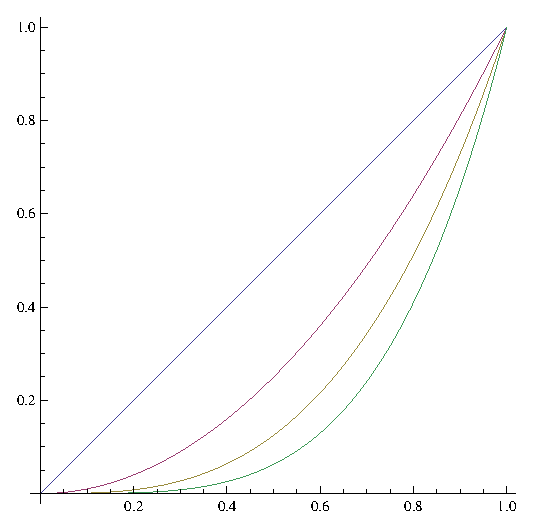
\includegraphics[width=0.3\textwidth]{fig/Template1n.eps}
    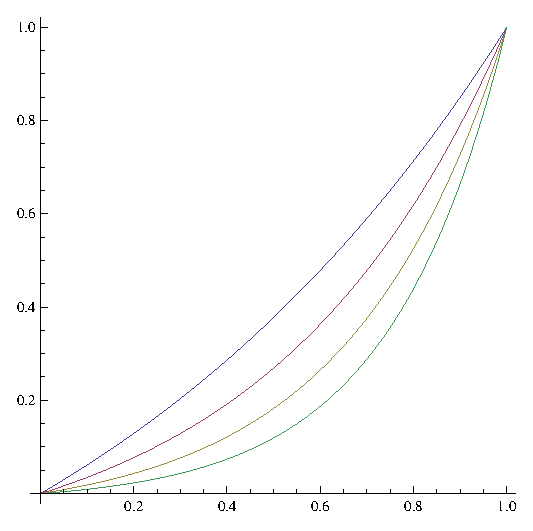
\includegraphics[width=0.3\textwidth]{fig/Template2n.eps}
    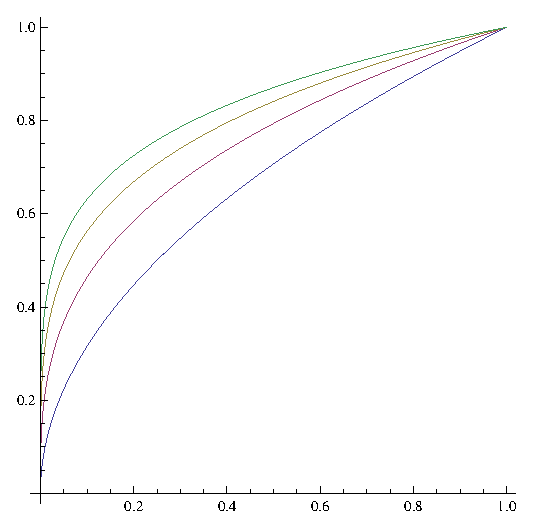
\includegraphics[width=0.3\textwidth]{fig/Template3n.eps}
  \end{center}
  \begin{center}
    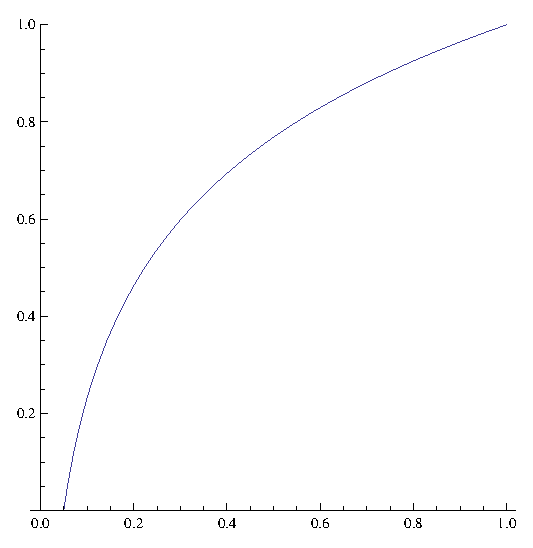
\includegraphics[width=0.3\textwidth]{fig/Template4n.eps}
    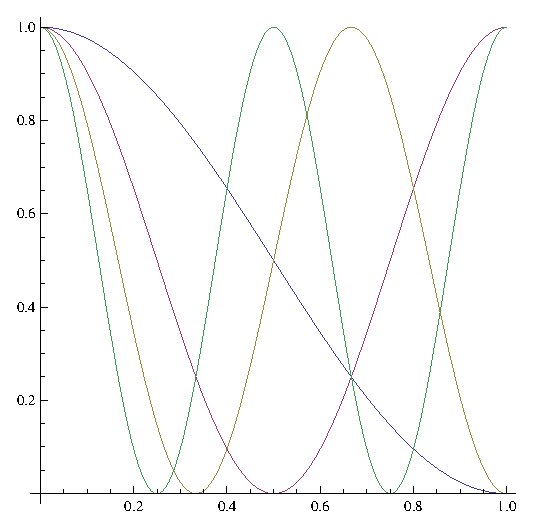
\includegraphics[width=0.3\textwidth]{fig/Template5n.eps}
    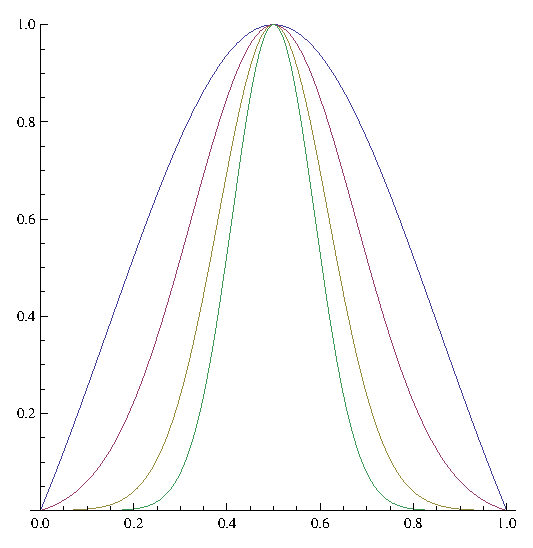
\includegraphics[width=0.3\textwidth]{fig/Template6n.eps}
  \end{center}
  \caption{\label{fig:classfct}Function templates used for supervised
    learning. $f_{1n},f_{2n},f_{3n}$ are shown in the upper row,
    $f_{4n},f_{5n},f_{6n}$ in the lower one. Normalization of
    logarithmic plots reduces them to the same shape.}
\end{figure*}

\subsubsection{Sampling of Input}
%% sampling of input
Input is given as an unordered list of
$\mathbf{r}_i=(x_i,y_i)\in\mathbb{R}^2$ values for datapoints, with
optional errors $\mathbf{e}_i=(e_i^x,e_i^y)\in\mathbb{R}^2$ in the
$x$- and $y$-direction. We do not want to perfectly fit the actual
points, probably with a polynomial of high order, but rather find a
curve that smoothly runs from point to point. This can be achieved
with a smearing of the inputs. Assuming Poissonian errors we could
sample each input by a set of $N$ points with Gaussian distribution in
both dimensions around the exact input value. This would additionally
account for the fact that an accumulation of points is rated higher,
and that big errors dilute the importance of the respective point.

We restrict ourself to equidistant sampling in $x$-direction such
that only $y$ values are to be learned, yielding a reduction of the
network size by a factor of roughly 2. This in turn implicates a reduction of
factor 4 for the connection weight matrices, ultimately effectuating a
speed-up in computation.

Several approaches sketched in the introduction work in Fourier space,
e.g. by clustering frequencies. This is not necessary for the simple
forward connected neural network that we chose here, a FFT thus being
developed only for use by a holographic neuron in follow-up work.

%
\subsubsection{Normalization of Input}
%% normalization of input
The raw data is transformed to lie in the range $[0,1]^2$ by translating with
%
\begin{eqnarray}\label{eq:translating}
	\mathbf{r}_i' &=& \mathbf{r}_i-\tilde{\mathbf{r}},\\
	\tilde{\mathbf{r}} &=& 	\begin{pmatrix}
					\min_i x_i\\
					\min_i y_i
			       	\end{pmatrix}
\end{eqnarray}
%
and scaling by
%
\begin{eqnarray}\label{eq:scaling}
	\mathbf{r}_i''&=& \mathbf{s}\cdot\mathbf{r}_i',\\
	\mathbf{e}_i''&=& \mathbf{s}\cdot\mathbf{e}_i',\\
	\mathbf{s}   &=& \begin{pmatrix}s^x\\s^y\end{pmatrix}
                      = \begin{pmatrix}
				1/(\max_i x_i-\min_i x_i)\\
				1/(\max_i y_i-\min_i y_i)
			\end{pmatrix},
\end{eqnarray}
%
A sample normalization acting upon a vector of positions with errors
is shown in table \ref{tab:ti1}.
%
%table of input before and after normalization
\begin{table}
\begin{center}
\begin{tabular}{lcllcl}\hline\hline
input&&&normalized&&\\
\hline
(87.901,16.033)&$\pm$&(1.217,3.629) & (0.935,0.069)&$\pm$&(0.014,0.042)\\
(47.201,56.778)&$\pm$&(5.137,0.619) & (0.466,0.542)&$\pm$&(0.059,0.007)\\
(18.216,20.656)&$\pm$&(1.553,2.618) & (0.132,0.123)&$\pm$&(0.018,0.030)\\
( 6.733,49.695)&$\pm$&(1.757,2.502) & (0.000,0.460)&$\pm$&(0.020,0.029)\\
(46.678,69.808)&$\pm$&(2.745,2.905) & (0.460,0.693)&$\pm$&(0.032,0.034)\\
(67.733,29.033)&$\pm$&(0.358,0.330) & (0.703,0.220)&$\pm$&(0.004,0.004)\\
(93.503,20.258)&$\pm$&(1.670,3.388) & (1.000,0.119)&$\pm$&(0.019,0.039)\\
(58.550,96.246)&$\pm$&(4.789,0.806) & (0.597,1.000)&$\pm$&(0.055,0.009)\\
(71.007,64.515)&$\pm$&(0.622,1.421) & (0.741,0.632)&$\pm$&(0.007,0.016)\\
(89.003,57.577)&$\pm$&(5.159,3.849) & (0.948,0.551)&$\pm$&(0.059,0.045)\\
(23.714,10.043)&$\pm$&(2.548,2.890) & (0.196,0.000)&$\pm$&(0.029,0.034)\\
(29.676,38.286)&$\pm$&(3.537,3.023) & (0.264,0.328)&$\pm$&(0.041,0.035)\\
\hline
\end{tabular}
\end{center}
\caption{\label{tab:ti1} Sample input before and after normalization.}
\end{table}

\subsection{Neural Network}
%network
\subsubsection{Basic Structure}
%% basic structure
From the available methods described in the appendix, we chose to
implement a simple forward connected network with two hidden layers
(cf. \ref{fig:network_topology}), following the script
\cite{Stoop2010}, p. 101. This network can divide the available
parameter space in several simply connected domains, which we need in
order to distinguish between a large number of function types
$f_{T,D}$. Additional hidden layers do not enhance the functionality
in a qualitative way; as a matter of fact the learning rate for
backpropagation would be compounded.

%fig of network
 \begin{figure}
   \begin{center}
     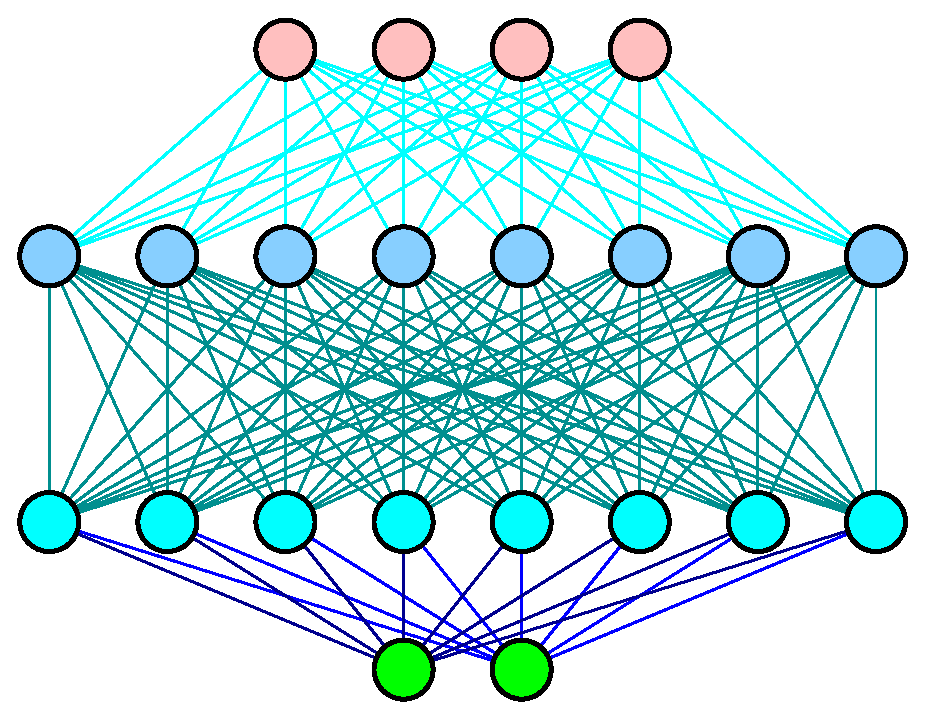
\includegraphics[width=0.45\textwidth]{fig/network_topology.eps}
   \end{center}
   \caption{\label{fig:network_topology}Basic topology of a forward
     connected network with two hidden layers. The shown configuration
     was used to map random input with 4 points at fixed
     $x$-coordinates to type and degree of the function, with the
     number of hidden neurons chosen such that the number of
     configurations to learn (4*4+1) is twice the number of
     neurons. Ability to classify noisy data is preserved.}
 \end{figure}
%
\subsubsection{Parameters}
%% parameters
Parameters in the network include number of hidden neurons,
distribution of starting connection weights, learning rate, output
function, and number of iterations. These will be investigated later
on. A parameter that is not investigated concerns the method of error
propagation through the network. Backpropagation with momentum,
resilient propagation, backpercolation, and QuickProp are only a few
which would enable faster convergence.

%output
\subsection{Output}
%% output of neural network
\subsubsection{Representation in Network}
The main output of the program is an equation $f(x)$ for the best
fitting function. This is achieved in two steps: first, the basic
function type and degree are determined, then they are put back into
unnormalized coordinates.

Our six function classes and all of the four degrees are stored
equidistantly in $[0,1]$ so as to maximize assignment quality. Another
trick to get better results with noisy data is the order in which the
input functions are stored: $f_{1D},f_{2D}$ and $f_{3D},f_{4D}$ do lie
next to each other, which ensures that the outputs for similar curves
do not differ much. This enhances the probability that rounding to the
next integer for function type ends up mostly in the surroundings of a
function that looks like the meant one.
%
%% error
\subsection{Error}
The basic error function to be minimized in order to find the function
type and degree is
%
\begin{equation}
  e=\sum_{i=1}^N (y_i-f(x_i))^2,
\end{equation}
%
taking into account the $y$-axis error only.

If we wanted a fit that includes $x$-direction as well for a
real-world application, we would use
%
\begin{equation}
  e=\sum_{i=1}^N (x_i-x_{m,i})^2+(y_{m,i}-f(x_{m,i})^2
\end{equation}
%
where $(x_{m,i},y_{m,i})$ denotes the coordinates of the nearest point
on the fitting curve to a given data point.
%
\subsubsection{Fitting, Backtransformation}
%% fitting from given formula
During normalization, scaling and translation parameters are stored
for later use. The fitted formula $\tilde{f}_{TD}(x)$ is then transformed back
%
\begin{equation}
  f(x)=t_y+s_y*\tilde{f}_{TD}(s_x*x+t_x)
\end{equation}
%
%
\subsection{Visualization}
% visualization
Visualization of the input data with error bars and fitting formula is
performed in the normalized coordinates, ranging over
$[0,1]\times[0,1]$ in the two-dimensional plane. See
fig. \ref{fig:vis} for a sample output.
%
%fig of sample input/visualization of fit
\begin{figure}
  \begin{center}
    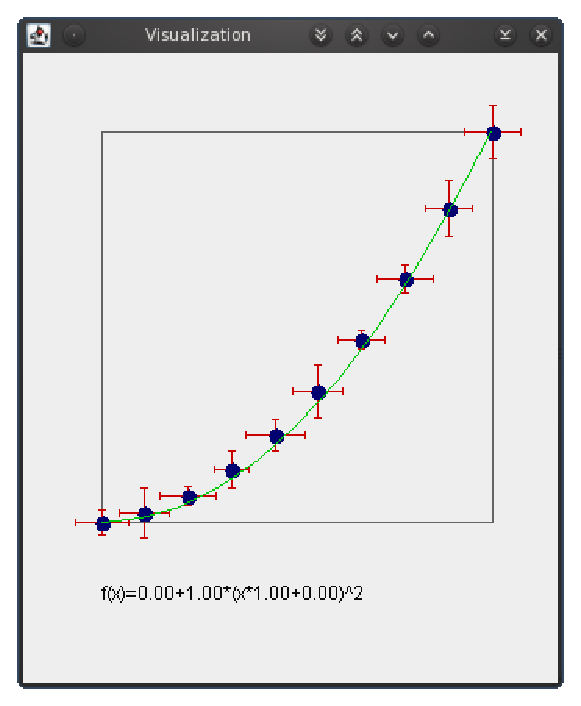
\includegraphics[width=0.3\textwidth]{fig/vis.eps}
  \end{center}
  \caption{\label{fig:vis}Sample visualization for fitting of an $x^2$}
\end{figure}

%implementation
\subsection{Implementation}
%%computation environment
\subsubsection{Computation environment}
The program is written in {\sc Java}, where we profited from
programming and debugging aids in the {\sc Eclipse}
environment. Visualization is accomplished with {\sc Swing} API. The
presented tests were run on an AMD Phenom 9750 processor using 64bit
registers and a total of 8GB RAM. Threading was not implemented, since
the crucial part of the program being backpropagation with online
updating would corrupt parallel computations.

%%program architecture
\subsubsection{Program Architecture}
Fig. \ref{fig:flow} gives an overview of the program architecture:
after choice of basic program mode, the training data is generated,
the network trained following \cite{Stoop2010}, and afterwards applied
different test input. Further data reduction needs error output to
external files; in all other cases online output of the found function
is sufficient.
%fig of flowchart, basic blocks
\begin{figure}
  \begin{center}
    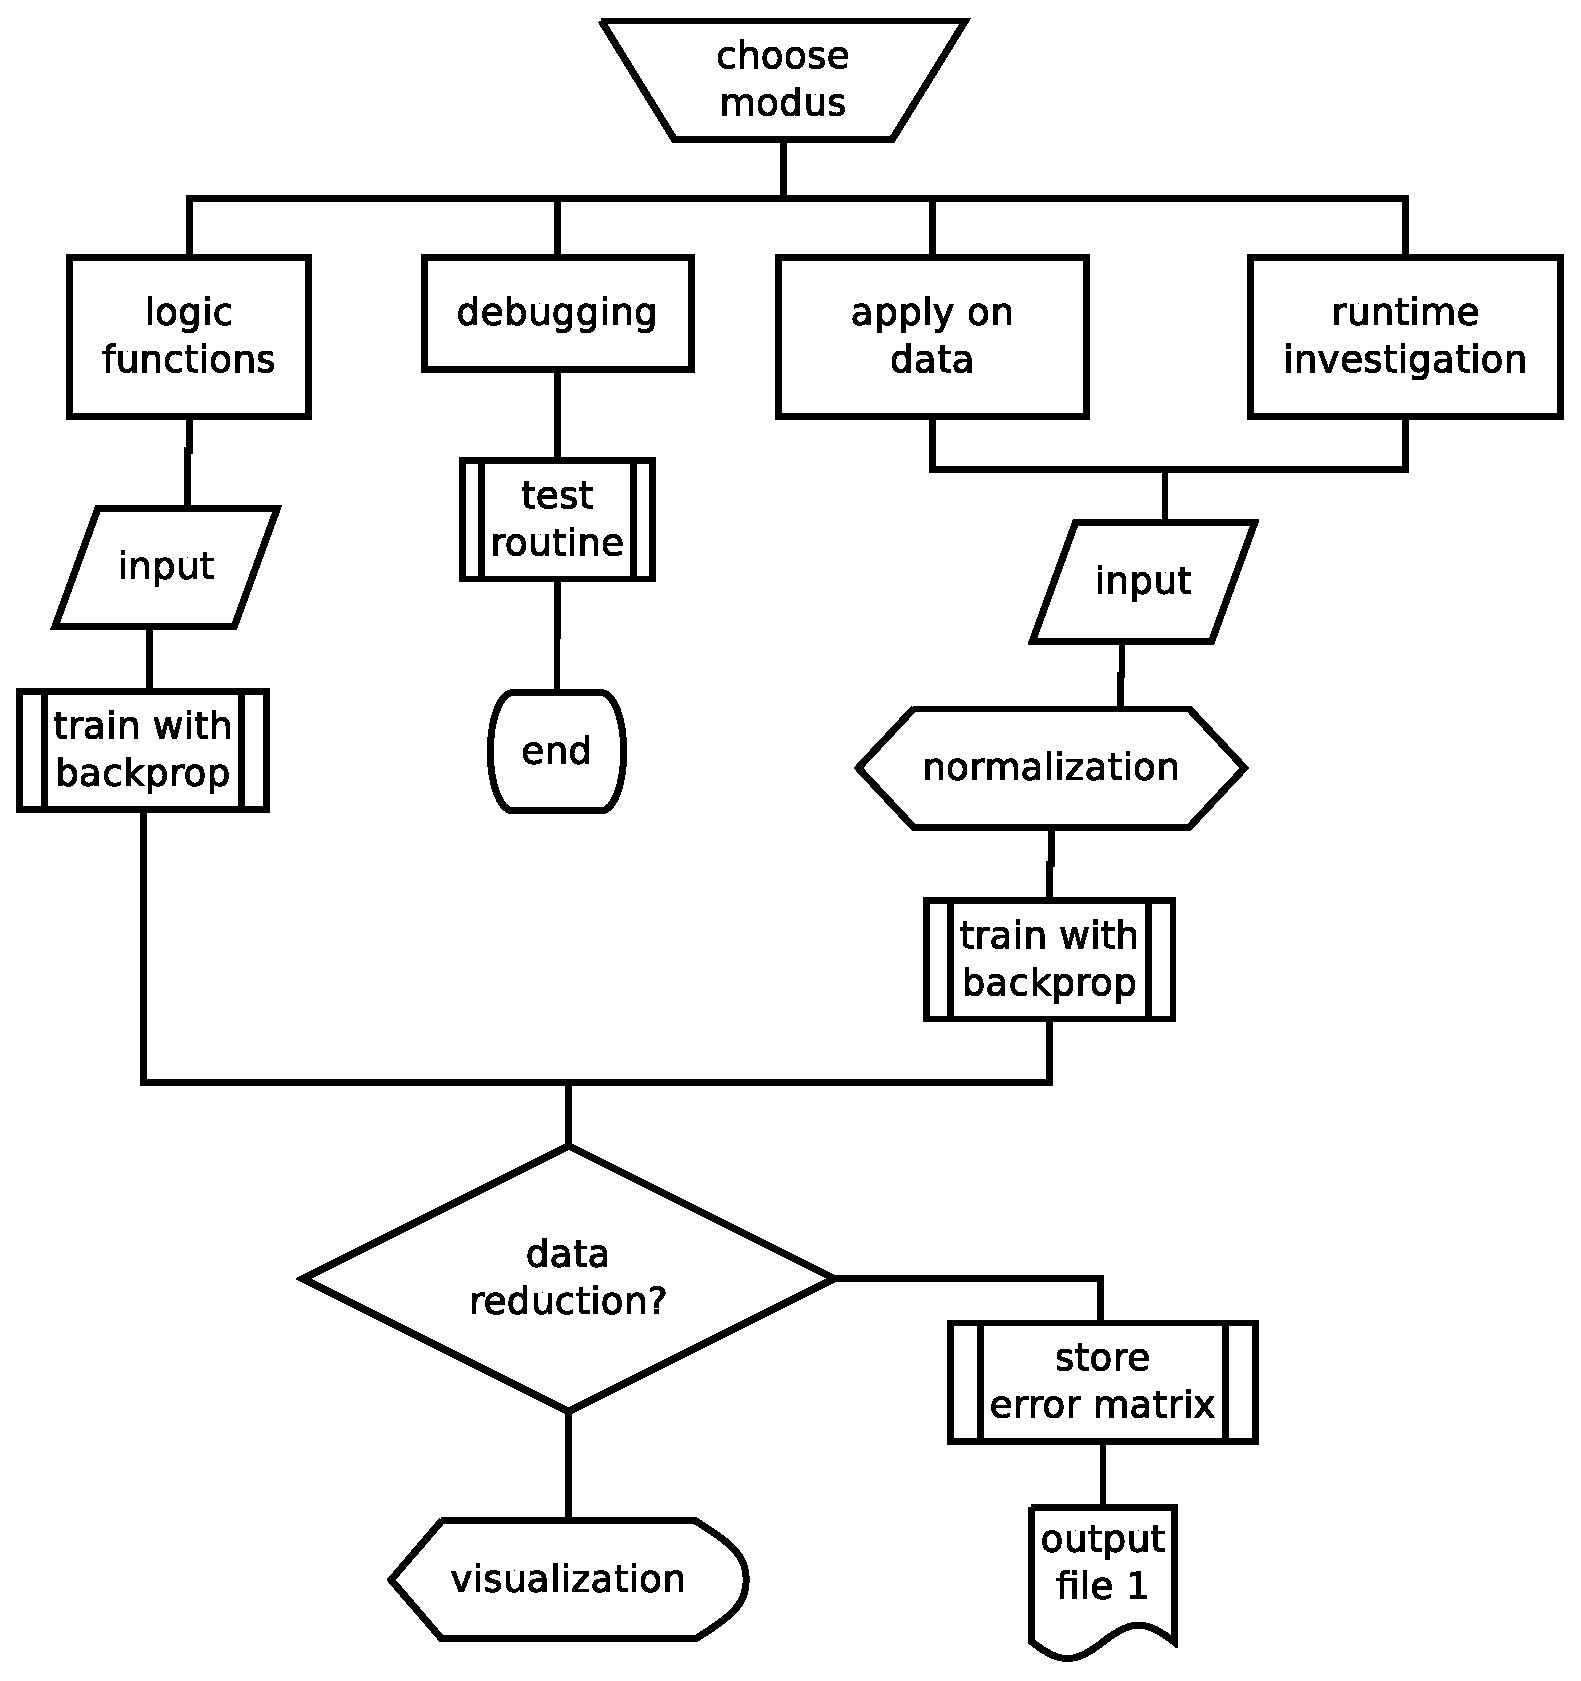
\includegraphics[width=0.45\textwidth]{fig/dia.eps}
  \end{center}
  \caption{\label{fig:flow}Basic architecture of {\rm Java} program}
\end{figure}
%
%
\section{Results}
\label{sec:Results}
%
%logic functions
\subsection{Logic Functions}
We let the neural network learn basic logic functions with two inputs
as a means to rule out basic errors. In the end, quite good
approximations were found with a network incorporating more than
$2*2+1$ hidden neurons in each layer, with strongest replication of
equal output values and weakest coincidence for the $\rm XOR$ and
${\rm NOT}({\rm XOR})$, see table \ref{tab:logic}.
%
% table with outputs for all logic functions with 2 inputs
\begin{table}\label{tab:logic}
\begin{center}
\begin{tabular}{rllll}\hline\hline
$(a,b)=(0,0)$&$(0,1)$&$(1,0)$&$(1,1)$&error $e$\\
\hline
0.0 & 0.0 & 0.0 & 0.0 & 0.0000\\
1.0 & 0.0 & 0.0 & 0.0 & 0.0005\\
0.0 & 1.0 & 0.0 & 0.0 & 0.0005\\
1.0 & 1.0 & 0.0 & 0.0 & 0.0004\\
0.0 & 0.0 & 1.0 & 0.0 & 0.0004\\
1.0 & 0.0 & 1.0 & 0.0 & 0.0003\\
0.0 & 1.0 & 1.0 & 0.0 & {\bf 0.0021}\\
1.0 & 1.0 & 1.0 & 0.0 & 0.0007\\
0.0 & 0.0 & 0.0 & 1.0 & 0.0009\\
1.0 & 0.0 & 0.0 & 1.0 & {\bf 0.0010}\\
0.0 & 1.0 & 0.0 & 1.0 & 0.0004\\
1.0 & 1.0 & 0.0 & 1.0 & 0.0005\\
0.0 & 0.0 & 1.0 & 1.0 & 0.0003\\
1.0 & 0.0 & 1.0 & 1.0 & 0.0004\\
0.0 & 1.0 & 1.0 & 1.0 & 0.0006\\
1.0 & 1.0 & 1.0 & 1.0 & 0.0000\\
\hline
\end{tabular}
\end{center}

\caption{\label{tab:logical} Output of neural network of size $(n_{\rm in},n_{\rm hidden,1},n_{\rm hidden,2},n_{\rm out})=(2,8,8,1)$ on all logic functions $f(a,b)$ after 1000 learning steps with $\eta=1.0$. Error is taken to be square of norm, $e=\sum_{i=1}^N(o-t)^2$.}
\end{table}
%
\subsection{Network applied on Training Set}
%training set
Using the neural network with 10 sample points, each 20 neurons on the
first and second hidden layer, learning rate 1.0 and sigmoid parameter
0.1, we get the values in table \ref{tab:td1} when applied to the
input dataset.

%table of output for all functions in training set
\begin{table}
\begin{center}
\begin{tabular}{llll}\hline\hline
type&degree&found type&found degree\\
\hline
1 & 1 & 0.968 & 1.018 \\
1 & 2 & 1.000 & 2.022 \\
1 & 3 & 1.024 & 3.035 \\
1 & 4 & 1.019 & 3.982 \\
\hline
2 & 1 & 2.003 & 1.016 \\
2 & 2 & 2.019 & 2.012 \\
2 & 3 & 1.983 & 2.989 \\
2 & 4 & 2.010 & 3.938 \\
\hline
3 & 1 & 2.955 & 1.041 \\
3 & 2 & 3.039 & 2.008 \\
3 & 3 & 2.972 & 3.029 \\
3 & 4 & 3.029 & 3.901 \\
\hline
4 & $1\ldots4$ & {\bf 4.001} & {\bf 2.587} \\
\hline
5 & 1 & 5.010 & 1.075 \\
5 & 2 & 5.026 & 2.065 \\
5 & 3 & 4.997 & 3.086 \\
5 & 4 & 4.991 & 3.974 \\
\hline
6 & 1 & 5.906 & 1.077 \\
6 & 2 & 5.965 & 2.089 \\
6 & 3 & 5.974 & 3.061 \\
6 & 4 & 5.938 & 3.946 \\
\hline
\end{tabular}
\end{center}
\caption{\label{tab:td1} Output of neural network applied on training data set.}
\end{table}
%
Most of the functions are classified correctly once the output values
are rounded to the nearest integer. An exception being degrees from
the logarithmic functions which are mapped to the same value, an expression
of the fact that a simple scaling and translation is undone
by normalization of the input values.
%
\begin{equation}
  \log(D\cdot x) = \log(x)+\log(D)\to\log(x)
\end{equation}
%

%
% quality measure
We define the quality of approximation in analogy to the logic
function example as as the difference to target value squared, either
from given output directly or after rounding to nearest
$n\in\mathbb{N}$.
%
\begin{eqnarray}
  e_1(T,D)&\equiv&(T-T_{{\rm tar}})^2+(D-D_{{\rm tar}})^2\\
  e_2(T,D)&\equiv&({\rm round}(T)-T_{{\rm tar}})^2+({\rm round}(D)-D_{{\rm tar}})^2
\end{eqnarray}
%
$T$ denotes type of function, $D$ is the degree. In notation of
eq. \ref{eq:class} the according function reads $f_{TD}(x)$.
%
%
\subsection{Parameter Dependence}
%parameter dependence
How does the performance of our network depend on the parameters? We
divide between parameters inherent to the neural network, as learning
rate, number of iterations, stretching of the sigmoid function and
measure of noise on the input?

\subsubsection{Noisy Input}
%noisy input
Noisy input is generated by taking the trained functions and adding noise, characterized by maximal disturbance $\delta$.
% 6 plots for each class, with four sets (degrees): errors
% e_1(solid line) and e_2(dotted line) as a function of noise
\begin{figure*}
  \begin{center}
   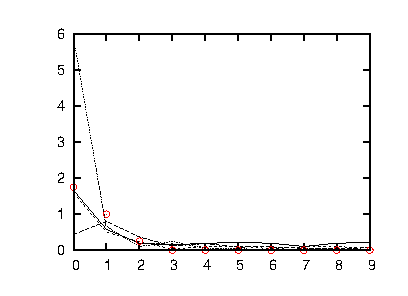
\includegraphics[width=0.3\textwidth]{fig/err/ea1.eps}
   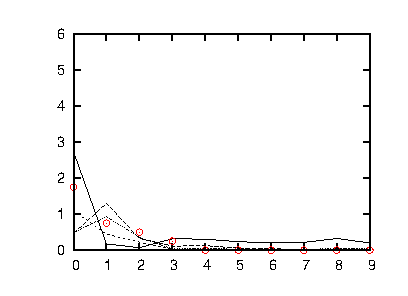
\includegraphics[width=0.3\textwidth]{fig/err/ea2.eps}
   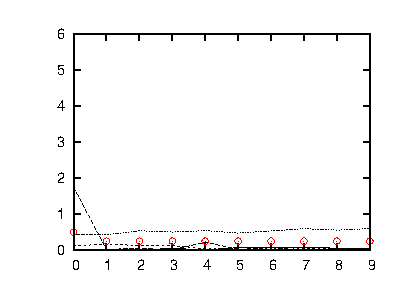
\includegraphics[width=0.3\textwidth]{fig/err/ea3.eps}
  \end{center}
  \begin{center}
   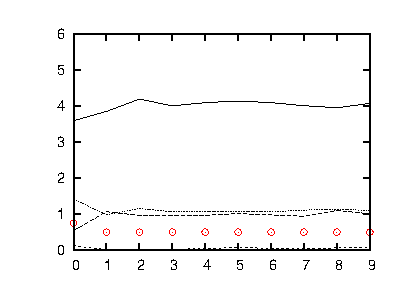
\includegraphics[width=0.3\textwidth]{fig/err/ea4.eps}
   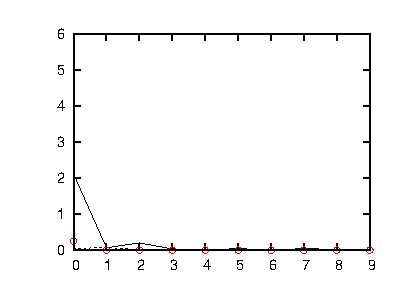
\includegraphics[width=0.3\textwidth]{fig/err/ea5.eps}
   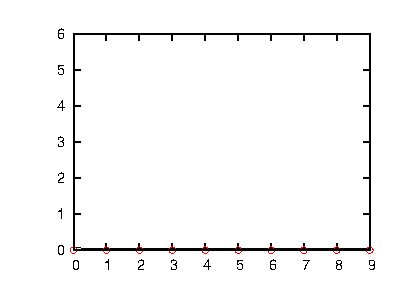
\includegraphics[width=0.3\textwidth]{fig/err/ea6.eps}
  \end{center}
  \caption{\label{fig:e12a}Classification error $e_1$ for each
    function as a function of noise is shown in black, where the label
    for the abscisse is $10(1-\delta)$ . Every panel holds all
    $f_{TD}$ for fix $T$. The red circles indicate $e2$ made by taking
    the rounded values for $T$ and $D$, averaged over all functions of
    a given type.}
\end{figure*}
%
Noise does only induce misclassification for
$f_{1D},f_{2D},f_{3D},f_{5D}$ if it is bigger than $\delta=0.08$. For $f_{4D}$ we do not expect small errors as all degrees should be mapped to one value. Interestingly there are no measurable effects of noise for the Gaussian distributions $f_{6D}$, at least up to $\delta=0.1$ they are well separated.


\subsubsection{Learning Rate and Number of Iterations}
%% learning rate
%% number of iterations

The error in classification does depend on the number of iterations, see fig. \ref{fig:e12nit} for the exact dependence broken down into the different function classes.
% fig of errors for each function class against number of iterations
\begin{figure*}
  \begin{center}
   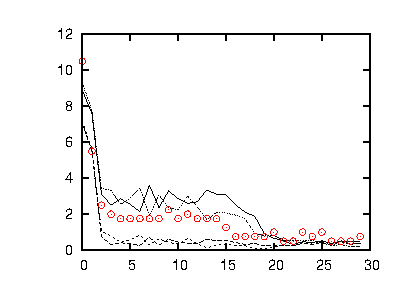
\includegraphics[width=0.3\textwidth]{fig/err/e1.eps}
   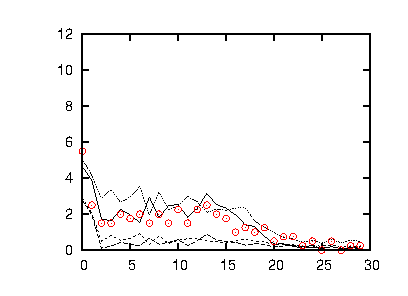
\includegraphics[width=0.3\textwidth]{fig/err/e2.eps}
   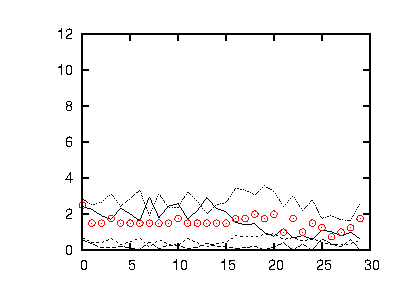
\includegraphics[width=0.3\textwidth]{fig/err/e3.eps}
  \end{center}
  \begin{center}
   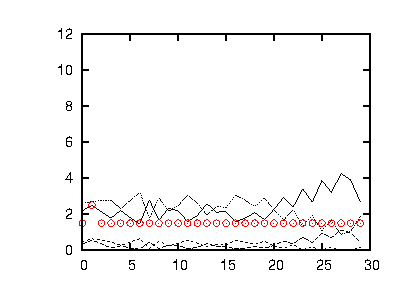
\includegraphics[width=0.3\textwidth]{fig/err/e4.eps}
   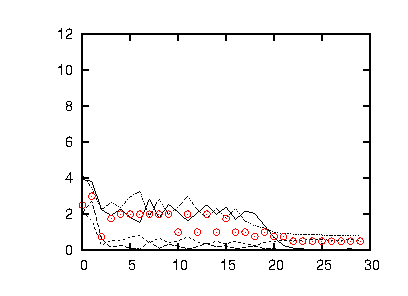
\includegraphics[width=0.3\textwidth]{fig/err/e5.eps}
   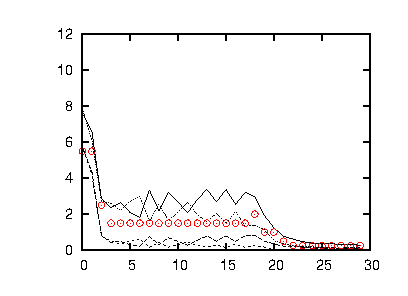
\includegraphics[width=0.3\textwidth]{fig/err/e6.eps}
  \end{center}
  \caption{\label{fig:e12nit}Classification error $e_1$ for each
    function as a function of learning steps is shown in black. Every
    panel holds all $f_{TD}$ for fix $T$. The values on the abscissa
    are scaled in 1000-steps. The red circles indicate $e2$ made by
    taking the rounded values for $T$ and $D$, averaged over all
    functions of a given type.}
\end{figure*}
%
We see that error is reduced in two steps: after the first 2000
iterations, approximately 3 out of 24 functions are classified
wrongly, this even holds when rounding is applied. After 20000 steps,
this is further reduced and almost every time the classification is
right for functions in $f_{1n},f_{2n},f_{5n},f_{6n}$. The errors
showing up in $f_{4n}$ are due to the fact that the degree cannot be
learned after normalization happens for the logarithmic function, the
type being mixed with $f_{3n}$ from the obvious marginal cases where
logarithmic and root functions look similar.

Learning rate and number of iterations is investigated next, with
results summarized in table \ref{tab:qof}. The trend for better
quality of fit with growing number of iterations discussed beforehands
is visible when considering the evolution for fixed $\eta$. Reading
the table along the other dimension, we find that worst recognition is
obtained with least lerning: the maxima of each row lie in the realm
of small learning rates. It is rapidly improved once $\eta=0.3$ is
encountered and stays mostly constant for larger values. Best results
are obtained for $\eta=0.9$ and not $\eta=1.0$, probably triggered by
the fact that this additional damping of oscillations around minima in
the error landscape during adjustment of connection weights helps to
converge faster. For the first part of convergence (the 2000 steps
mentioned before) this is not relevant, though; it is only after 4000
steps that full propagation of the adjustments causes a temporal rise
of classification error.
% table of quality against learning rate, and nit
\begin{table*}
\begin{center}
\begin{tabular}{r|rrrrrrrrrr}\hline\hline
$N_{it}=$&1&$2$&$3$&$4$&$5$&$6$&$7$&$8$&$9$&$10$\\
\hline
$\eta=0.1$&98.3&85.0&45.3&34.3&33.8&33.8&33.7&33.7&33.8&34.1\\
$\eta=0.2$&77.6&35.1&34.2&33.7&33.7&33.5&33.3&32.7&29.3&20.1\\
$\eta=0.3$&34.4&33.6&33.4&32.5&22.3&14.1&13.5&13.2&12.5&11.8\\
$\eta=0.4$&33.9&33.6&33.0&21.8&14.2&12.8&11.4&10.5&10.3&10.4\\
$\eta=0.5$&33.8&33.9&33.3&19.5&13.4&12.6&11.3&10.2&10.5&10.2\\
$\eta=0.6$&33.7&33.4&19.5&12.8&12.5&13.2&10.2&10.1& 9.3& 9.8\\
$\eta=0.7$&33.6&31.0&12.9&11.5&11.1&10.3&10.3& 8.9& 9.6& 9.4\\
$\eta=0.8$&34.2&33.2&13.5&12.0&11.4&10.4&10.1&10.8& 8.5& 9.9\\
$\eta=0.9$&33.4&14.1&11.6&10.6& 9.3& 8.5& 7.8& 7.1& 6.6& 6.5\\
$\eta=1.0$&34.3&14.3&12.0&10.7&12.5&10.3& 9.3& 9.5&10.4& 9.7\\
\hline
\end{tabular}
\end{center}
\caption{\label{tab:qof}Overall classification error as function of learning rate $\eta\in[0.1,1.0]$ and number of iterations $N_{{\rm it}}=n_{{\rm it}}/10^4\in[1,10]$.}
\end{table*}
%
\subsubsection{Shape of Sigmoid Function}
%
So far, the intuitive parameters for convergence were examined. A
simple adaptation of the network working on logical functions to the
function classification scheme by mere scaling did not work, even when
experimenting with different choices of learning rate and number of
iterations. The reason was that the biggest impact on learning
efficiency comes from stretching the sigmoidal output function of each
neuron, which is in fact so strong that it easily can suppress any
progression to completion. The first runs of the neural network
yielded no result due to the fact that random initial values for the
connection weights add up for a large number of neurons in one layer
and are mapped by the vanilla sigmoid function to a value
$1+\epsilon$, $\epsilon\ll1</math>$. Only if the sigmoid function is
stretched by setting small $a$ in
%
\begin{equation}
  {\rm sig}_a(x)\equiv\frac{1}{1+\exp(-ax)}
\end{equation}
%
the changes in weight get bigger than machine precision. Our
preliminary choice of $a=0.1$ still requires the high number of 25000
iterations per input pattern to get approximately 90\% of the
functions recognized correctly. In fig. \ref{fig:ea} the effect of
simoidal steepness $a$ on classification error after $10^6$
iterations. As long as $a<0.9$, there is hope for actual recognition,
best for some values around $a\approx0.2$.
% fig of quality against sigmoid parameter for fixed nitmax, eta
\begin{figure}
  \begin{center}
    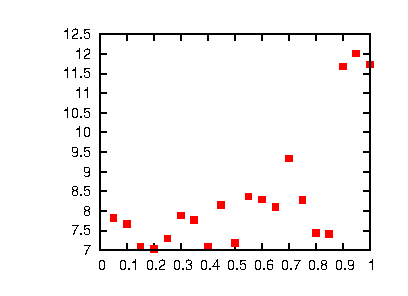
\includegraphics[width=0.45\textwidth]{fig/err/ea.eps}
  \end{center}
  \caption{\label{fig:ea}Total classification error $e$ as a function of sigmoid parameter $a$, with fixed $\eta=0.9$ and $n_{it}=10^6$.}
\end{figure}
%
\subsubsection{Number of Hidden Neurons}
%% runtime characteristics if number of hidden neurons is changed
The number of hidden neurons on both layers are kept at the same
value. Varying this number has both impacts on quality of fit and
runtime, see \ref{tab:run}.
\begin{table}
\begin{center}
\begin{tabular}{rll}\hline\hline
$n_{{\rm hid,1,2}}$&$e$&$t[{\rm s}]$\\
\hline
 1&86.23& 1.7\\
 2&30.56& 1.9\\
 3&14.84& 2.5\\
 4&12.38& 2.9\\
 5& 9.31& 3.5\\
 6&10.79& 4.0\\
 7&10.00& 4.7\\
 8& 9.32& 5.3\\
 9& 9.33& 6.0\\
10& 7.32& 6.7\\
\hline
15& 7.64&11.3\\
\hline
20& 6.58&17.5\\
\hline
\end{tabular}
\end{center}
\caption{\label{tab:run}Dependence of quality of fit after $10^5$ iterations on number of hidden neurons, together with runtime characteristics.}
\end{table}
%
\subsection{Limitations}
%limitations
Limitations of our code mainly arise from the degeneracies of several
functions. Additional heuristic knowledge needs to be implemented in
order to let the network propose ''simple'' function forms.
%
\section{Discussion}
\label{sec:Discussion}
%
%
\subsection{Summary}
We presented the architecture of a program to simulate a neural
network with two hidden layers, aiming at classification of a set of
basic functions. Introducing a measure for the quality of fit allowed
us to investigate dependence on different parameters. Learning
efficiency is foremost influenced by the sigmoidal output function
form. Little noise does not influence most fits. Learning parameter
and number of iterations need a short sample run to find the optimal
values; the learn parameter should be a little less than unity to
allow efficient error minimization. A tradeoff between accuracy of fit
for the training functions, generality and computing resources leads
to a choice for the number of hidden neurons; twice the input number
is a starting point.
%
%
\subsection{Enhancements}
The environment is prepared to scale to more sampling points, random
input, to find a whole linear superposition of fitting formulae to
approach the data even further. The proposed methods can moreover be
generalized for fitting parametric functions to three-dimensional
datasets. A possible extension would search for formulae of arbitrary
two-dimensional surfaces, or even try to classify three-dimensional
objects in topological classes.

\section{Acknowledgments}
\label{sec:Acknowledgments}
%
I would like to thank Ruedi Stoop for stimulating discussions and for
creating such a pleasant atmosphere in class. Stefan Martignoli gave
numerous hints how to implement algorithms in {\sc Mathematica}, which
was helpful to get a working knowledge on backpropagation.

%
% end of content
%

% table template
%\begin{table}
%\begin{center}
%\begin{tabular}{rlrlc}\hline\hline
%a&b&c&d&e\\
%\hline
%s&o&m&e&t\\
%m&o&r&e&t\\
%\hline
%\end{tabular}
%\end{center}
%\caption{\label{tab:td1} Output of neural network applied on training data set.}
%\end{table}
%
%
% sample figure inclusion statements
%
% \begin{figure}
%   \begin{center}
%     \includegraphics[width=0.45\textwidth]{fig/label}
%   \end{center}
%   \caption{\label{fig:label}small figure, width one column}
% \end{figure}
%
% spanning two columns
% 
% \begin[ht]{figure*}
%   \begin{center}
%     \hspace{1cm}
%     \includegraphics[width=0.85\textwidth]{fig/label}
%   \end{center}
%   \caption{\label{fig:label}big figure, width one page}
% \end{figure*}
%
%
\bibliography{main}
%
\label{lastpage}
\end{document}